\documentclass[12pt, letterpaper] {article}

\parindent=5mm
\usepackage[spanish]{babel}

\usepackage{amssymb}
\usepackage{amsmath} 
\usepackage{amsfonts}

\usepackage[numbers,sort&compress]{natbib}
\usepackage{graphicx}

\usepackage{url}
\usepackage{hyperref}

\usepackage[top=25mm, bottom=20mm, left=1.5cm, right=1.5cm]{geometry}
\setlength{\parskip}{2mm}
\setlength{\parindent}{1pt}

\usepackage{listings}

\usepackage{float}

\usepackage[utf8]{inputenc}
\usepackage{graphicx} 
\usepackage{subfigure} 

\usepackage{color}
\usepackage{multirow}

\definecolor{dkgreen}{rgb}{0,0.6,0}
\definecolor{gray}{rgb}{0.5,0.5,0.5}
\definecolor{mauve}{rgb}{0.58,0,0.82}

\usepackage[table,xcdraw]{xcolor}

\usepackage{color}
\usepackage{listings}
\lstset{ %
  language=R,                     % the language of the code
  basicstyle=\footnotesize,       % the size of the fonts that are used for the code
  numbers=left,                   % where to put the line-numbers
  numberstyle=\tiny\color{gray},  % the style that is used for the line-numbers
  stepnumber=1,                   % the step between two line-numbers. If it's 1, each line
                                  % will be numbered
  numbersep=5pt,                  % how far the line-numbers are from the code
  backgroundcolor=\color{white},  % choose the background color. You must add \usepackage{color}
  showspaces=false,               % show spaces adding particular underscores
  showstringspaces=false,         % underline spaces within strings
  showtabs=false,                 % show tabs within strings adding particular underscores
  frame=single,                   % adds a frame around the code
  rulecolor=\color{black},        % if not set, the frame-color may be changed on line-breaks within not-black text (e.g. commens (green here))
  tabsize=2,                      % sets default tabsize to 2 spaces
  captionpos=b,                   % sets the caption-position to bottom
  breaklines=true,                % sets automatic line breaking
  breakatwhitespace=false,        % sets if automatic breaks should only happen at whitespace
  title=\lstname,                 % show the filename of files included with \lstinputlisting;
                                  % also try caption instead of title
  keywordstyle=\color{blue},      % keyword style
  commentstyle=\color{dkgreen},   % comment style
  stringstyle=\color{mauve},      % string literal style
  escapeinside={\%*}{*)},         % if you want to add a comment within your code
  morekeywords={*,...}            % if you want to add more keywords to the set
} 


\author{Ricardo Rosas Macías}

\title{Práctica 12: red neuronal}

\date{\today}

\begin{document}

\maketitle


\section{Introducción}
La red neuronal es un modelo que funciona de una forma similar y simplificada a la de un cerebro humano, en un ordenador. Este tipo de inteligencia artificial permite obtener una solución con la ayuda de criterios de utilidad, a través de la combinación de parámetros y ponderaciones de entrenamiento de selección multi-objetivo; asistidos de perceptrónes, que favorecen la identificación de la posición, de modo que favorecen discernir la predicción del híperplano. 

 \section{Objetivo}
Para llevar acabo el objetivo de la práctica, se hizo un proceso de aprendizaje de patrones, con los cuales la red neuronal fuera capaz de crear ponderaciones sinápticas para la elección correcta del resultado. Asimismo, se paralelizó el experimento para obtener un mejor desempeño en los tiempos de ejecución del código.
 
 \subsection{Descripción}
 
La finalidad del experimento es \cite{elisawebRN}:
\begin{quotation}
 ``Paralelizar un segmento del código y estudiar de manera sistemática el desempeño de la red neuronal para los diez dígitos en función de las tres probabilidades asignadas a la generación de los dígitos (ngb), variando a las tres en un experimento factorial adecuado.

Para el primer reto, se extiende y entrena la red neuronal para que reconozca además por al menos doce símbolos ASCII adicionales, aumentando la resolución de las imágenes a $5\times7$ de lo original de $3\times5$ (modificando las plantillas de los dígitos acorde a este cambio).''
\end{quotation}

\section{Resultados y conclusiones}

De acuerdo a la literatura anteriormente reportada \cite{PAP12}, se hicieron líneas de código que permitieran una ejecución paralela. De igual manera, se cuantificó el tiempo que toma en realizar la ejecución del código y se comparo con la ejecución normal, como se muestra en la parte inferior.

\begin{lstlisting}[language=R]
repetitions <- 30
trainNP <- microbenchmark(
  for (t in 1:5000) { 
    d <- sample(0:tope, 1)
    pixeles <- runif(dim) < modelos[d + 1,]
    correcto <- binario(d, n)
    for (i in 1:n) {
      w <- neuronas[i,]
      deseada <- correcto[i]
      resultado <- sum(w * pixeles) >= 0
      if (deseada != resultado) {
        ajuste <- tasa * (deseada - resultado)
        tasa <- tranqui * tasa
        neuronas[i,] <- w + ajuste * pixeles
      }
    }
  }
  , times = repetitions, unit = "s")

testNP <- microbenchmark({
  contadores <- matrix(rep(0, k*(k+1)), nrow=k, ncol=(k+1))
  rownames(contadores) <- 0:tope
  colnames(contadores) <- c(0:tope, NA)

  for (t in 1:300) {
    d <- sample(0:tope, 1)
    pixeles <- runif(dim) < modelos[d + 1,] 
    correcto <- binario(d, n)
    salida <- rep(FALSE, n)
    for (i in 1:n) {
      w <- neuronas[i,]
      deseada <- correcto[i]
      resultado <- sum(w * pixeles) >= 0
      salida[i] <- resultado
    }
    r <- min(decimal(salida, n), k) 
    contadores[d+1, r+1] <- contadores[d+1, r+1] + 1
  }
}
, times = repetitions, unit = "s")

newrons <- function(i, neuronas, pixeles)
newr <- function(){
  d <- sample(0:tope, 1)
  pixeles <- runif(dim) < modelos[d + 1,] 
  
  salida <- sapply(1:n, neuronas[i,])
  r <- min(decimal(salida, n), k)
  return(c(d+1, r+1))
}
suppressMessages(library(doParallel))
clust <- makeCluster(detectCores()-1)
registerDoParallel(clust)

testP <- microbenchmark({
  contadores <- matrix(rep(0, k*(k+1)), nrow=k, ncol=(k+1))
  rownames(contadores) <- 0:tope
  colnames(contadores) <- c(0:tope, NA)
  conta <- foreach(t = 1:300, .combine = "rbind", .export = c("tope", "dim", "modelos", "neuronas", "pixeles")) %dopar% newr()
  for (i in 1:300){
    contadores[conta[i, 1], conta[i, 2]] <- contadores[conta[i, 1], conta[i, 2]] + 1
  }
}
, times = repetitions, unit = "s")

stopCluster(clust)
trains <- cbind("Normal" = trainNP$time)
tests <- cbind("Paralelizada" = testP$time, "Normal" =testNP$time)
\end{lstlisting}

Se realizó una visualización gráfica con ayuda de la paquetería \textit{ggplot2}, como se muestra en la figura \ref{PS}, en la cual se observa claramente un aumento de tiempos al realizar la ejecución normal, de modo que permite definir que la ejecución paralela es mejor para el experimento. 

\begin{figure}[H]
\centering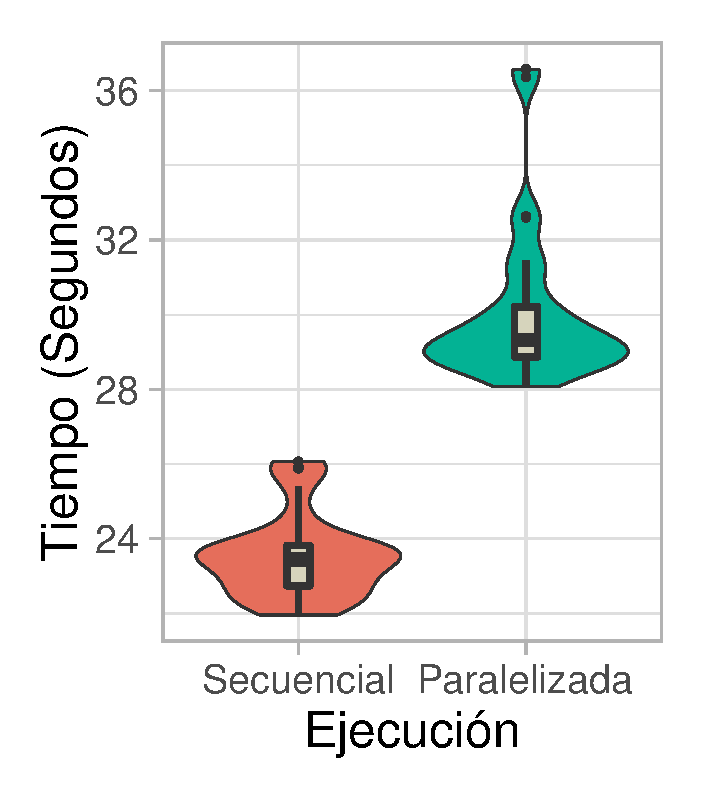
\includegraphics[width=90mm]{Tejec.eps}
\caption{Tiempo de tarda la ejecución del código}
\label{PS}
\end{figure}

Acorde al precedente \cite{PAP12}, se hicieron líneas de código que proporcionen el desempeño de la red neuronal para los diez dígitos. Por ende, en el código inferior, se determinó una variación de las probabilidades de color los pixeles; de manera que permita observar el desempeño de la red neuronal a estos cambios. 

\begin{lstlisting}[language=R]
newrons <- function(i, neuronas, pixeles){
  w <- neuronas[i,]
  return(sum(w * pixeles) >= 0)
} 
newr <- function(){
  d <- sample(0:tope, 1)
  pixeles <- runif(dim) < modelos[d + 1,]
  correcto <- binario(d, n)
  salida <- sapply(1:n, newrons, neuronas, pixeles)
  r <- min(decimal(salida, n), k) 
  return(c(d+1, r+1))
}

Negros <- c(0.90, 0.95, 0.995)
Grises <- c(0.80, 0.90, 0.992)
Blancos <- c(0.002, 0.02, 0.1)

data <- data.frame("Porcen"=numeric(), "N" = numeric(), "G" = numeric(), "B"= numeric())
for (negro in Negros){
  for (gris in Grises) {
    for (blanco in Blancos){
      
 modelos <- read.csv("digitos.modelo.csv", sep=" ", header=FALSE, stringsAsFactors=F)
      modelos[modelos=='n'] <- negro
      modelos[modelos=='g'] <- gris
      modelos[modelos=='b'] <- blanco

      suppressMessages(library(doParallel))
      clust <- makeCluster(detectCores()-1)
      registerDoParallel(clust)
      
      contadores <- matrix(rep(0, k*(k+1)), nrow=k, ncol=(k+1))
      rownames(contadores) <- 0:tope
      colnames(contadores) <- c(0:tope, NA)
      conta <- foreach(t = 1:300, .combine = "rbind", .export = c("tope", "dim", "modelos", "neuronas", "pixeles")) %dopar% newr()
      for (i in 1:300){
        contadores[conta[i, 1], conta[i, 2]] <- contadores[conta[i, 1], conta[i, 2]] + 1
      }
      stopCluster(clust)

      atino <- numeric()
      noatino <- numeric()
      for (i in 1:(dim(contadores)[1])){
        noatino[i] <- 0
        for (j in 1:(dim(contadores)[2])){
          if(i == j){
            atino[i] <- contadores[i,j]
          } else {
            noatino[i] <- sum(noatino[i], contadores[i,j])
          }
        }
      }
      porcen <- numeric()
      for (i in 1:length(atino)){
        porcen[i] <- noatino[i]/(atino[i]+noatino[i])
        por <- c(porcen[i], negro, gris, blanco)
        data <- rbind(data, por)
      }
    }
  }
}
\end{lstlisting}

Por consiguiente, se obtuvieron los resultados del código anterior gráficamente, en la figura \ref{PSQT}, en donde se puede observar como un gran porcentaje de error de cada dígito se encuentra muy cerca de la normalidad. Por lo cual, se procedió a realizar un análisis de varianza; para obtener información más detallada, cómo se muestra en el cuadro \ref{CRR}, en el cual se aprecia un mayor efecto en las probabilidades de los píxeles negros y blancos, en atención a lo cual los pixeles blancos cuentan con mayor relevancia, debido a la mayor influencia de clasificación. 

\begin{figure}[H]
\centering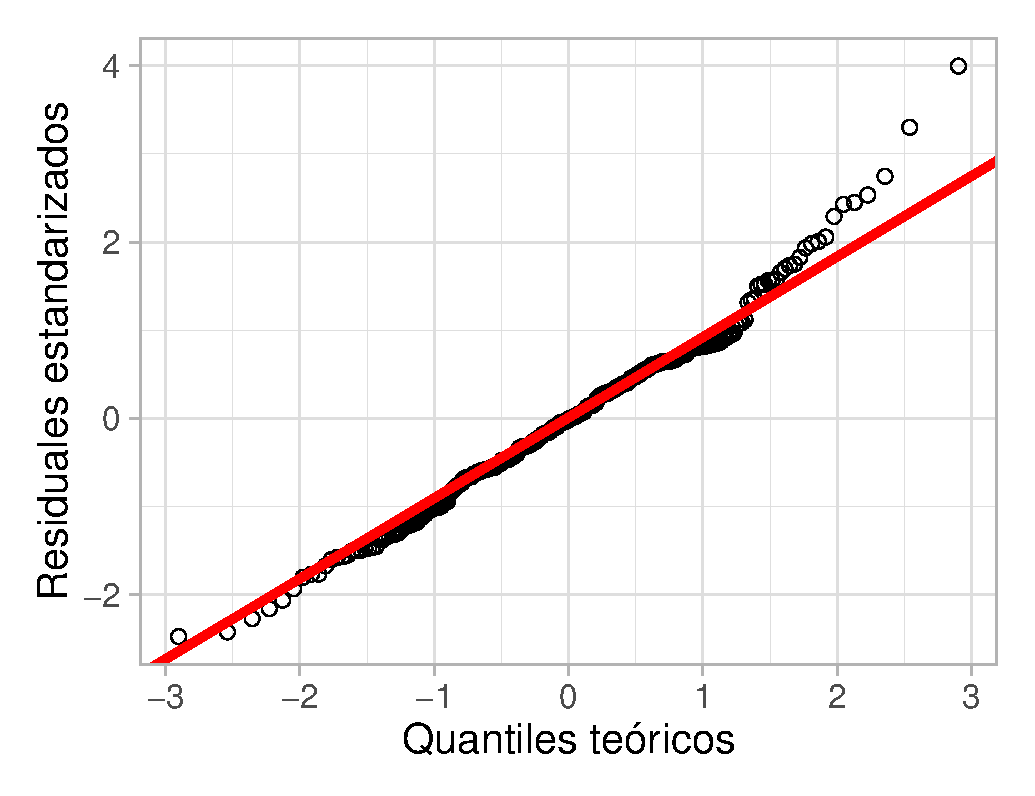
\includegraphics[width=90mm]{TEvalnorm.eps}
\caption{Evaluación de normalidad}
\label{PSQT}
\end{figure}

Por otro lado, en el cuadro \ref{CRR} se observa una diferencia estadísticamente significativa en el ``Valor F'' de 19.408 y 172.176 los píxeles Negro y blanco respectivamente; en comparación al gris, de manera que cuentan con mayores grados de libertad como se muestra en la columna  ``Df'', así como con un un valor  ``Pr'' por debajo de 0.05, que indica una menor desviación estándar. De modo que se puede concluir que hay un incremento en la probabilidad de presencia en los píxeles Blancos. 

\begin{table}[H]
\centering\caption{Resultados de análisis de varianza}\label{CRR}
\begin{tabular}{|l|l|l|l|l|l|}
\hline
\rowcolor[HTML]{EFEFEF} 
\multicolumn{1}{|c|}{\cellcolor[HTML]{EFEFEF}{\color[HTML]{333333} \textbf{}}} & \multicolumn{1}{c|}{\cellcolor[HTML]{EFEFEF}\textbf{Df}} & \multicolumn{1}{c|}{\cellcolor[HTML]{EFEFEF}\textbf{Sum Sq}} & \multicolumn{1}{c|}{\cellcolor[HTML]{EFEFEF}\textbf{Media Sq}} & \multicolumn{1}{c|}{\cellcolor[HTML]{EFEFEF}\textbf{valor F}} & \multicolumn{1}{c|}{\cellcolor[HTML]{EFEFEF}\textbf{Pr(\textgreater{}F)}} \\ \hline
\rowcolor[HTML]{ECF4FF} 
{\color[HTML]{333333} Negro}                                                   & {\color[HTML]{333333} 2}                                 & {\color[HTML]{333333} 1.435}                                 & 0.718                                                         & 19.408                                                        & 1.52e-08                                                                  \\ \hline
\rowcolor[HTML]{ECF4FF} 
{\color[HTML]{333333} Gris}                                                    & {\color[HTML]{333333} 2}                                 & {\color[HTML]{333333} 0.502}                                 & 0.251                                                         & 6.792                                                         & 0.00135                                                                   \\ \hline
\rowcolor[HTML]{ECF4FF} 
{\color[HTML]{333333} Blanco}                                                  & {\color[HTML]{333333} 2}                                 & {\color[HTML]{333333} 12.732}                                & 6.366                                                         & 172.176                                                       & \textless{}2e-16                                                          \\ \hline
\rowcolor[HTML]{ECF4FF} 
Negro:Gris                                                                     & 4                                                        & 0.020                                                        & 0.005                                                         & 0.138                                                         & 0.96800                                                                   \\ \hline
\rowcolor[HTML]{ECF4FF} 
Negro:Blanco                                                                   & 4                                                        & 0.245                                                        & 0.061                                                         & 1.657                                                         & 0.16067                                                                   \\ \hline
\rowcolor[HTML]{ECF4FF} 
Gris:Blanco                                                                    & 4                                                        & 0.678                                                        & 0.170                                                         & 4.586                                                         & 0.00138                                                                   \\ \hline
\rowcolor[HTML]{ECF4FF} 
Negro:Gris:Blanco                                                              & 8                                                        & 0.183                                                        & 0.023                                                         & 0.617                                                         & 0.76287                                                                   \\ \hline
\rowcolor[HTML]{ECF4FF} 
Residuals                                                                      & 243                                                      & 8.984                                                        & 0.037                                                         &                                                               &                                                                           \\ \hline
\end{tabular}
\end{table}


\subsection{Reto 1}

Con ayuda de la literatura \cite{PLP12} se realizó un documento CSV que se muestra en la parte inferior, en las cuales con la ayuda de la codificación de color para cada pixel, permitió realizar una resolución de imagen de $5\times7$ y reconocimiento de símbolos ASCII.

\begin{lstlisting}[language=R]
n g n g n g b b b g n b b b n g b b b g n b b b n g b b b g n g n g n
n n g b b b b n b b b b n b b b b g b b b b n b b b b n b b n n g n n
n g g n g b b b b g b b b b n g g n g g n b b b b g b b b b g n g g n
g n g n g b b b b n b b b b g g n g n n b b b b g b b b b n g n g n g
g g b g g n n b n n g g b g g n n g n n b b b g g b b b n n b b b g g
g n n g g g b b b b n b b b b n g g n n b b b b g b b b b g n g g n n
g n g n g n b b b b g b b b b n g n g n g b b b g n b b b n g n g n g
n g n g n b b b b g b b b b n b b g n g b b b b n b b b b g b b b b n
n g n g n g b b b g n b b b n g n g n g n b b b n g b b b g n g n g n
g n g n g n b b b n g b b b g n g n g n b b b b g b b b b n b b b b g
n n b b b g g b b b n n b b b g g b b b n n b b b g g g g g n n n n n
n g n g n g n g n g b b n b b b b g b b b b n b b g n g n g n g n g n
n g n g n g n g n g n g b b b g n b b b n g b b b g n g n g n g n g n
g g b g g n n b n n g g b g g n n n n n g g b g g n n b n n g g b g g
g n g n g n g n g n b b g b b b b n b b b b g b b b b n b b b b g b b
n g n g n g n g n g n g b b b g n g n b n g b b b g n g n g n g n g n
n n n n n n n n n n n n b b b n n n b b n n b b b n n b b b n n b b b
n n b n n g g b g g n n b n n g g b g g n n b n n g g g g g n n n n n
g n g n g n b b b n g b b b g n g n g n g b b b b n b b b b g b b b b
n g n g n n b b b n g b b b g n n g n n g b b b g n b b b n n b b b n
n b b b n g b b b g n b g b n g b n b g g b n b g n b g b n g g n g g
g n g n g n b n b n g b g b g n b n b n g b g b g n b b b n g b b b g
\end{lstlisting}

\begin{lstlisting}[language=R]
modelos <- read.csv("digitosext.modelo.csv", sep=" ", header=FALSE, stringsAsFactors=F)

r <- 7
c <- 5
dim <- r * c

n <- 49
w <- ceiling(sqrt(n))
h <- ceiling(n / w)

SASCIIAD <- c(0:9, "U", "L", "I", "C", "H", "M", "T", "P", "A", "W", "E", "F",)

png("plantilla.png", width=1600, height=2000)
par(mfrow=c(w, h), mar = c(0,0,7,0))
suppressMessages(library("sna"))

for (j in 1:n) {
  d <- sample(0:21, 1)
  pixeles <- runif(dim) < modelos[d + 1,] 
  imagen <- matrix(pixeles, nrow=r, ncol=c, byrow=TRUE)
  plot.sociomatrix(imagen, drawlab=FALSE, diaglab=FALSE, 
                   main=paste(SASCIIAD[d+1], ""), cex.main=5)
}
graphics.off()
\end{lstlisting}

En la figura \ref{Plant} se observa la plantilla con los números 0--9 y con los símbolos ASCII, generada con la ejecución del código.

\begin{figure}[H]
\centering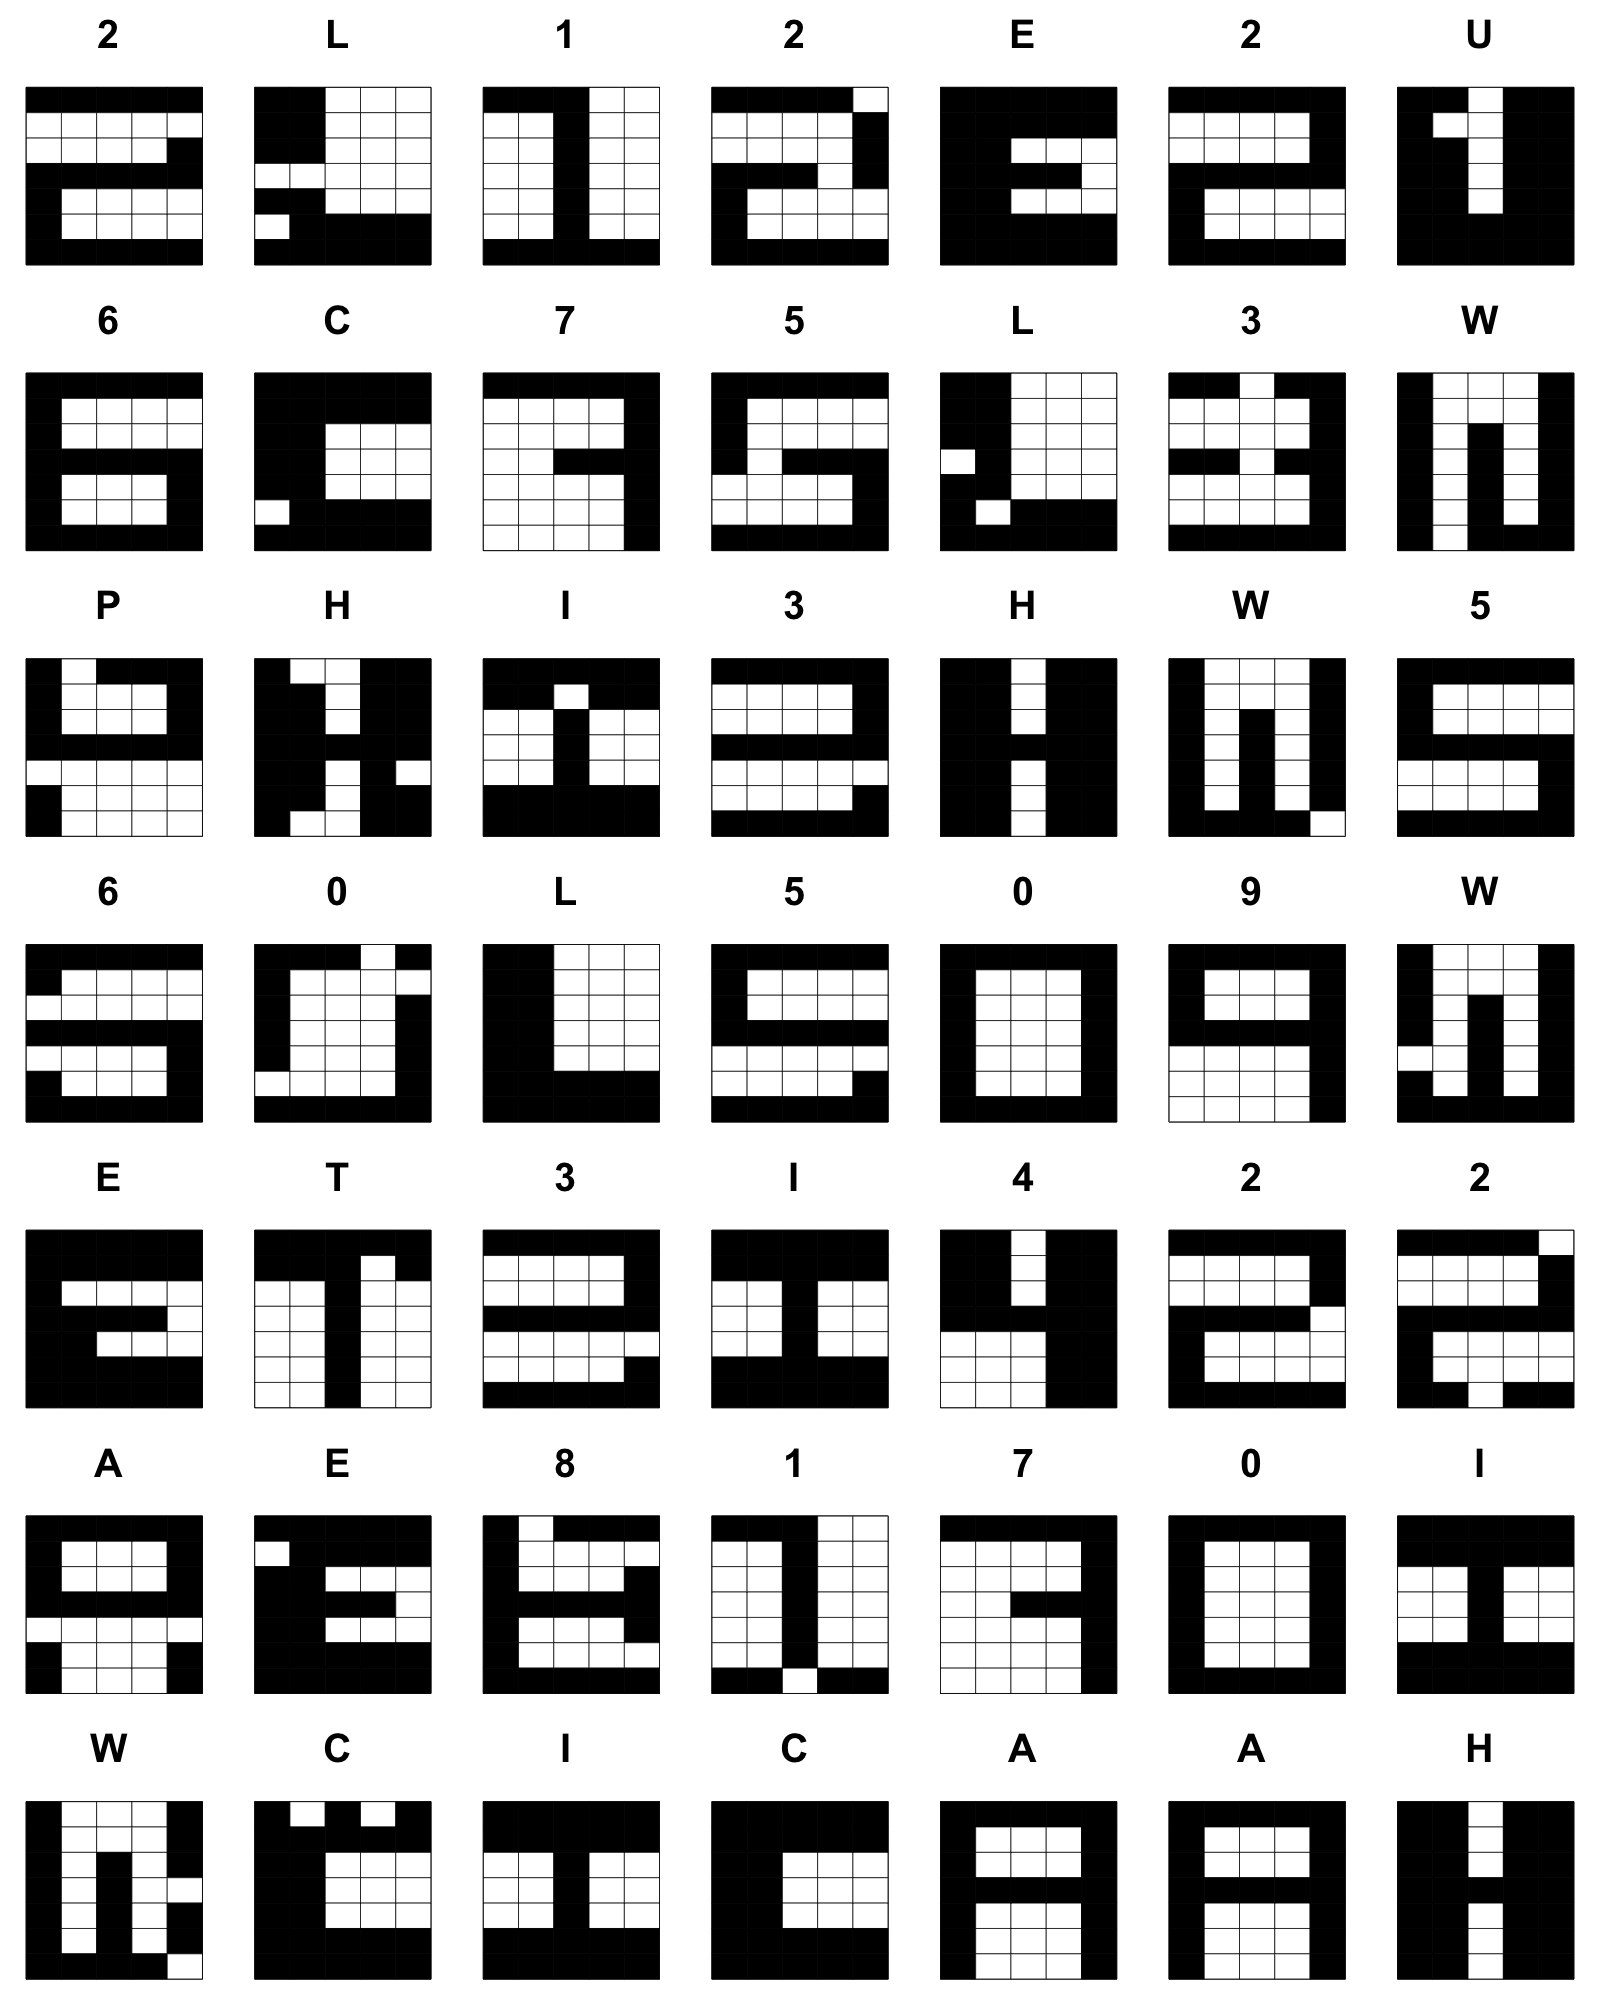
\includegraphics[width=90mm]{plantilla.png}
\caption{Plantilla con símbolos ASCII adicionales de $5\times7$}
\label{Plant}
\end{figure}



\bibliographystyle{plainnat}

\bibliography{BiblioHWP12}

\end{document}